\chapter{Objective Assessment}
\label{chap:objective}
This chapter contains the development process of the Face Quality Analysis application. To start we will look at functional and non-functional requirements followed by a use cases. Further, we include sequence diagrams to show how some of the core functionality work. To the end we will have an insight in the design and implementations phase followed by results on the datasets provided by the FIQMs.

\section{Requirements}
When approaching the requirements, we had to make decisions based on the task description  as well as the meetings with Mobai. The description and our colleagues were open in terms of setting requirements, but some core concepts of the desired product were simplicity, clarity, performance and modifiability. Based on these principles, we (along with Mobai) shaped non-functional and functional requirements. Also, as mentioned in Section \ref{sec:OurModel} not all requirements were set at the start of the project, so they had to be fine-tuned and confirmed along the development process. This did not mean that any important change in the software occurred, but as more functionality were suggested, requirements had to be created to describe them. The \textbf{non-functional} requirements describes how the software should perform. These are the following requirements:
\begin{itemize}
    \item The application should be deployed in a container.
    \item The architecture should consist of backend and frontend.
    \item APIs should be implemented as REST APIs.
    \item The application should make it easy to add new FIQMs.
\end{itemize}
The \textbf{functional} requirements defines what the software should do or not do. These are the following requirements:
\begin{itemize}
    \item The application should run every available FIQM.
    \item The application should run all FIQMs together.
    \item The application should return a sheet with quality scores on every image based on the FIQMs as a JSON file.
    \item If only one images is evaluated, the image should be displayed with corresponding different attribute scores. 
\end{itemize}

\subsection{What type of application}
The responsibility of choosing application type was given to the bachelor group. Selecting either a web or desktop application was challenging, but we carefully evaluated the type of application that suited our needs the best. 

\subsubsection*{Desktop application}
Since desktop applications are downloaded to your operating system, they are available independently whether you are connected to the internet or not. In that way it is possible to stay functional all the time \cite{WebVsDesktop}. The constant accessibility that desktop applications provide automatically make them more secure. In a way, you never have to be connected to the internet when working on tasks which reduces the possibility of being hacked by a margin. Having a fast computer would be beneficial running a desktop application. The application uses memory and CPU which returns a good user experience given a resourceful computer. However, using an old computer would not be a problem either. The fact that desktop applications allows for running older versions of the program with all functional availability does not make a hardware upgrade necessary. Also, given that desktop apps do not coerce to update the software make it adaptable to choose a suitable version for the computer's specifications. It is also uncomplicated to store files from the application, as information are supported by the computer's hard drives. 

Although, desktop applications have their downsides. The application may require multiple updates to enable full functionality which seems persistent and unnecessary. If the work is performed on different devices, each device need the same installation to synchronize the progress. This will also make it more challenging for multiple users to collaborate on desktop applications. Another disadvantage with a desktop application is the dependence of operating system requirements. To allow the latest functionality the application provides, specific requirements are required. 

\subsection*{Web application}
A web application only require one installation step before the software is workable \cite{WebVsDesktop}. This is very time saving in terms of web applications make updates behind the scenes and the only simple thing to do is to type the internet address into the browser. All updates are free and immediately available. The ease of availability for these applications make synchronizing with several devices a small case. In addition to this, the simplicity of managing cooperation with different users is remarkable. Some licence issues may arise, but this solution makes people collaborate from their permanent working stations. Another advantage is the application's accessibility. It is possible to acquire web applications from any browser or operating system. 

However, web applications do not offer offline mode which requires a constant internet connection. In addition, the application's capability hardly depends on the internet connection and speed. A poor connection and speed result in a bad workflow. As regular updates could be beneficial, are there less possibilities of using and older versions of the software. 

\subsection*{Our application}
We chose to build a web application as our approach. Mobai did not need to run the application in offline mode, since they always had sufficient internet connection. Also, because many employers would work on the web page at the same time, it should be easy to manage multiple users so they can work on their required working stations. 

\section{Use case}
We have created a use case diagram to show the core functionality and activities within the application. The diagram was build from the perspective of the user (described in Section \ref{sec:TargetGroups}) which were employees at Mobai. The cases differ in complexity where running all metrics would be the most challenging. That is because it includes running every metric and providing scores for each image. 

\begin{figure}[h]
    \centering
    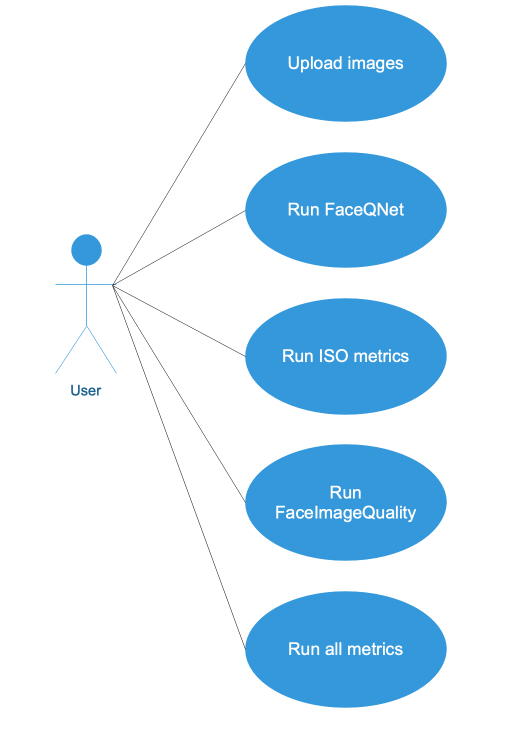
\includegraphics[scale = 0.3]{figures/UseCaseDiagram.png}
    \caption{Use case diagram}
    \label{fig:UseCase}
\end{figure}

\newpage

\begin{table}[h]
\centering
\resizebox{\textwidth}{!}{%
\begin{tabular}{|p{12cm}|} 
\hline
\textbf{Use case:} Upload images\\
\textbf{Actor:} User \\
\textbf{Goal:} Upload selected images \\
\textbf{Description:} The user can select which images he would like to upload to the application. Images will only be stored in the application for that session. \\ \hline
\end{tabular}%
}
\end{table}


\begin{table}[h]
\centering
\resizebox{\textwidth}{!}{%
\begin{tabular}{|p{12cm}|} 
\hline
\textbf{Use case:} Run ISO metrics\\
\textbf{Actor:} User \\
\textbf{Goal:} Evaluate images with the ISO metric \\
\textbf{Description:} After uploading selected images, the user would push ''Run ISO metrics'' to assess the images. The application returns a sheet with quality scores for each facial image. \\ \hline
\end{tabular}%
}
\end{table}

\begin{table}[h]
\centering
\resizebox{\textwidth}{!}{%
\begin{tabular}{|p{12cm}|} 
\hline
\textbf{Use case:} Run FaceQNet\\
\textbf{Actor:} User \\
\textbf{Goal:} Evaluate images with the FaceQNet \\
\textbf{Description:} After uploading selected images, the user would push ''Run FaceQNet'' to assess the images. The application returns a sheet with quality scores for each facial image. \\ \hline
\end{tabular}%
}
\end{table}

\newpage

\begin{table}[h]
\centering
\resizebox{\textwidth}{!}{%
\begin{tabular}{|p{12cm}|} 
\hline
\textbf{Use case:} Run FaceImageQuality\\
\textbf{Actor:} User \\
\textbf{Goal:} Evaluate images with the FaceImageQuality \\
\textbf{Description:} After uploading selected images, the user would push ''Run FaceImageQuality'' to assess the images. The application returns a sheet with quality scores for each facial image. \\ \hline
\end{tabular}%
}
\end{table}


\begin{table}[h]
\centering
\resizebox{\textwidth}{!}{%
\begin{tabular}{|l|p{9cm}|} 
\hline
\textbf{Case} & Run all metrics  \\ \hline
\textbf{Description} & The user runs all metrics in the applications which returns scores for every image.      \\ \hline
\textbf{Basic Flow} &   \begin{enumerate}
    \item The user pushes the upload images button.
    \item The user navigates to select wanted images to perform the metrics on.
    \item After uploading images, the user presses ''Run all metrics''
    \item The program returns a sheet with quality scores of the selected images
\end{enumerate}     \\ \hline
\textbf{Alternative} &  The user runs all metrics without uploading any images
            \begin{enumerate}
                \item The application displays an error and asks the user to upload images.
            \end{enumerate}
The user presses reset before running the metrics 
            \begin{enumerate}
                \item Uploading images again is necessary.
            \end{enumerate}
                    \\  \hline
\textbf{Pre-condition} & The application is running. \\ \hline
\textbf{Post-condition} &  Images that are being evaluated are uploaded. \\ \hline
\end{tabular}%
}
\caption{High level use case for ''Run all metrics''}
\end{table}

\newpage
\section{Sequence diagrams}
Two sequence diagrams, one high level and one low level, will be showcased and discussed. Our web application is simple in design, but behind the scenes several entities are interacting with each other. To firmly understand how the application is constructed, it is essential to acknowledge the interaction between the components. Sequence diagrams are convenient easy to read tools to visualize a given interaction within a time sequence. Providing both high and low level sequence diagrams will yield a complete picture of our system from a surface to an in-depth level.

\subsection{High level - ISO metric}

\begin{figure}[h]
    \centering
    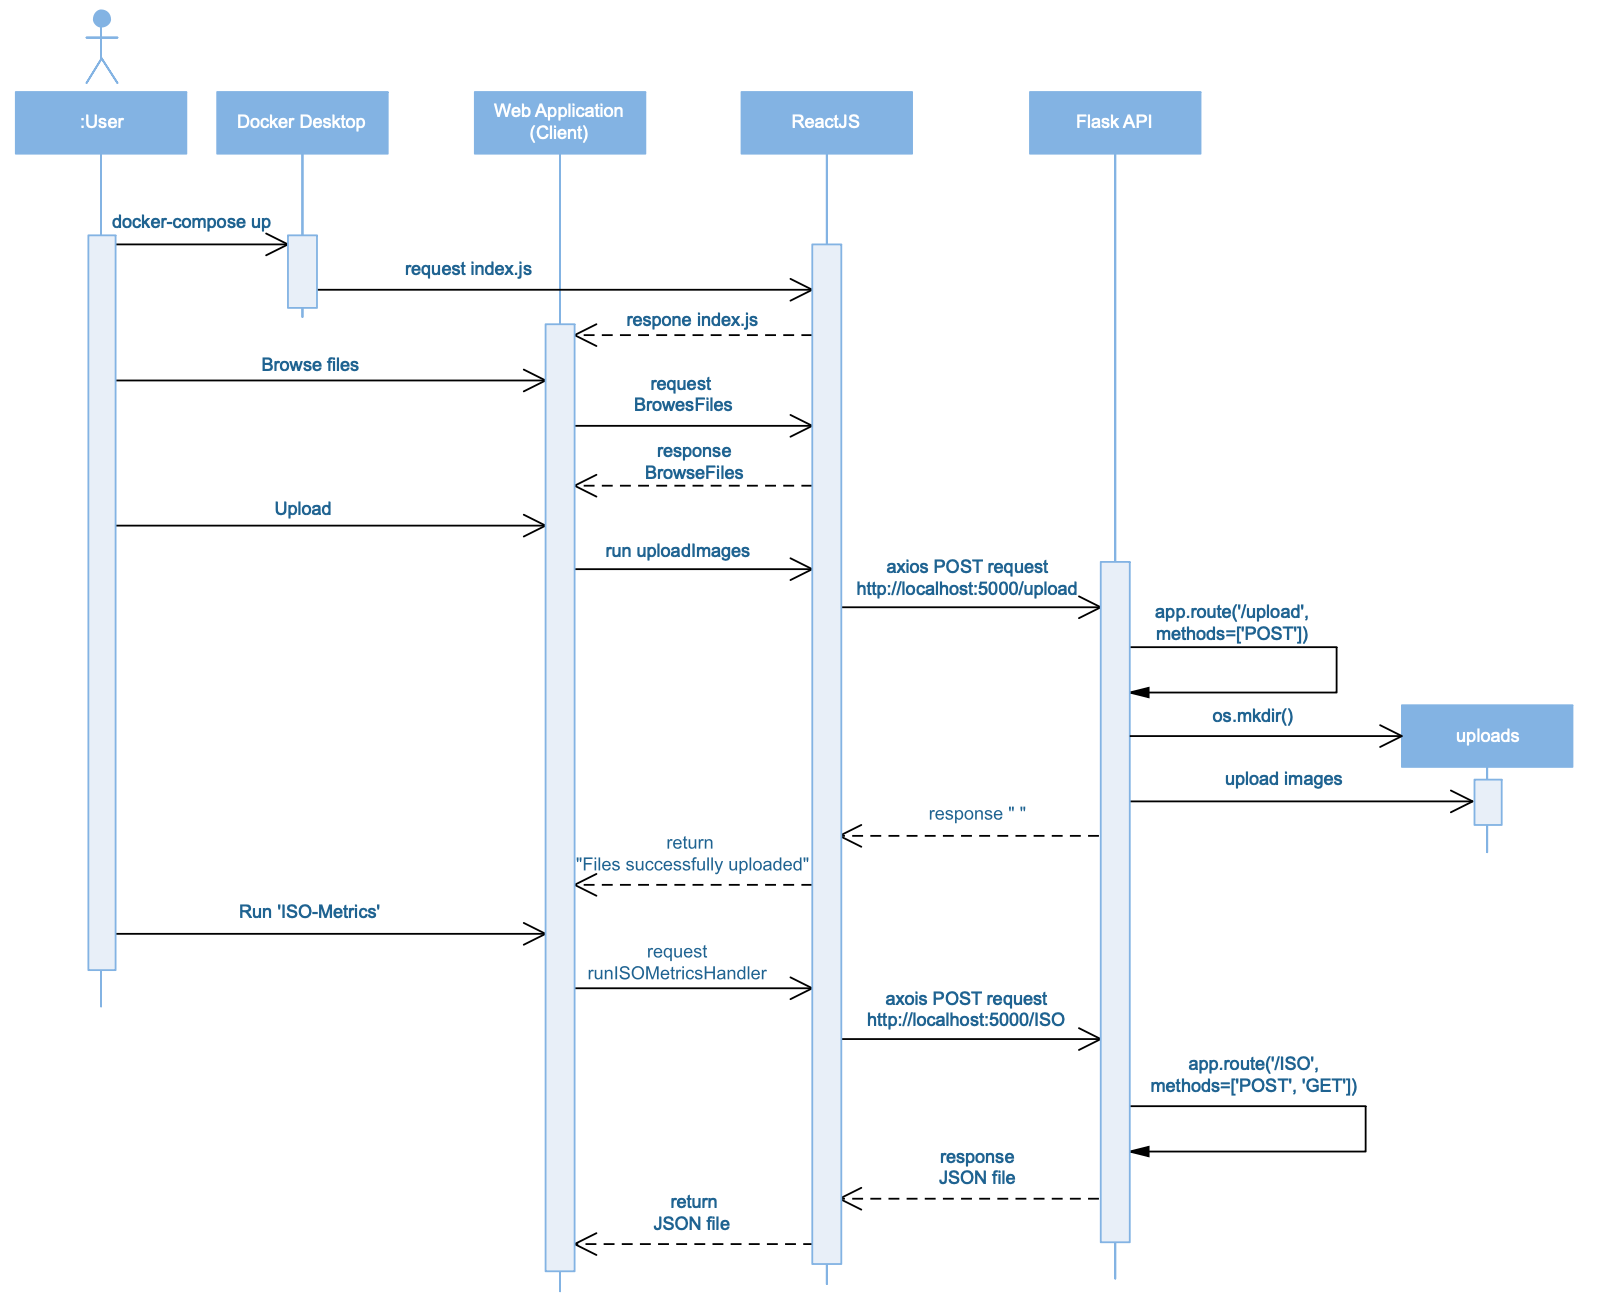
\includegraphics[scale = 0.52]{figures/HighLevel.png}
    \caption{ISO metric: high level sequence diagram}
    \label{fig:highlevel}
\end{figure}
\newpage
Figure \ref{fig:highlevel} is meant as a surface level visualization of what happens the first time the application is started on a new computer and a metric is executed. After the two docker images are pulled from Docker Hub, the application is now ready to run. From the terminal window the command: ``docker-compose up'', will boot up both the react and flask servers. An immediate request to render the index.js file in the web application is sent to the react server. After the home page is displayed in the web browser the user can press a button to browse files, which will send a request to the react server to open a window of your local files. Images are now ready to be selected. The selected images are stored in a state that waits for the ``Upload'' button to be pressed. Once the user presses the button a function called uploadImages will be executed from the react server that in return redirects an axios http POST request to the external flask backend API at port 5000. The POST request contains all the selected images. An API by the name of ``upload'' saves all selected images in a specified uploads folder in the backend before it is redirected back to the react server that displays a ``Files successfully uploaded'' message to the web application. Since this is the first time the application is executed, the uploads folder has not yet been created. The upload API therefore has to create it before uploading the images and returning to the web application. 

Once the images are saved in the backend, the web application is now ready to execute any metric. The button ``Run `ISO-Metrics''' on the web page is clicked which requests the function runISOMetricsHandler to be executed from the react server. This function will likewise redirect an axios POST request to port 5000. An API by the name of ISO will receive the request which triggers the API to execute ISO-metric. Once the metric has generated quality scores on the uploaded images, it returns a single JSON file that contains the scores. This JSON file is returned to the react server which in return displays the scores on the web page. 
\newpage

\subsection{Low level - FaceQNet}

\begin{figure}[h]
    \centering
    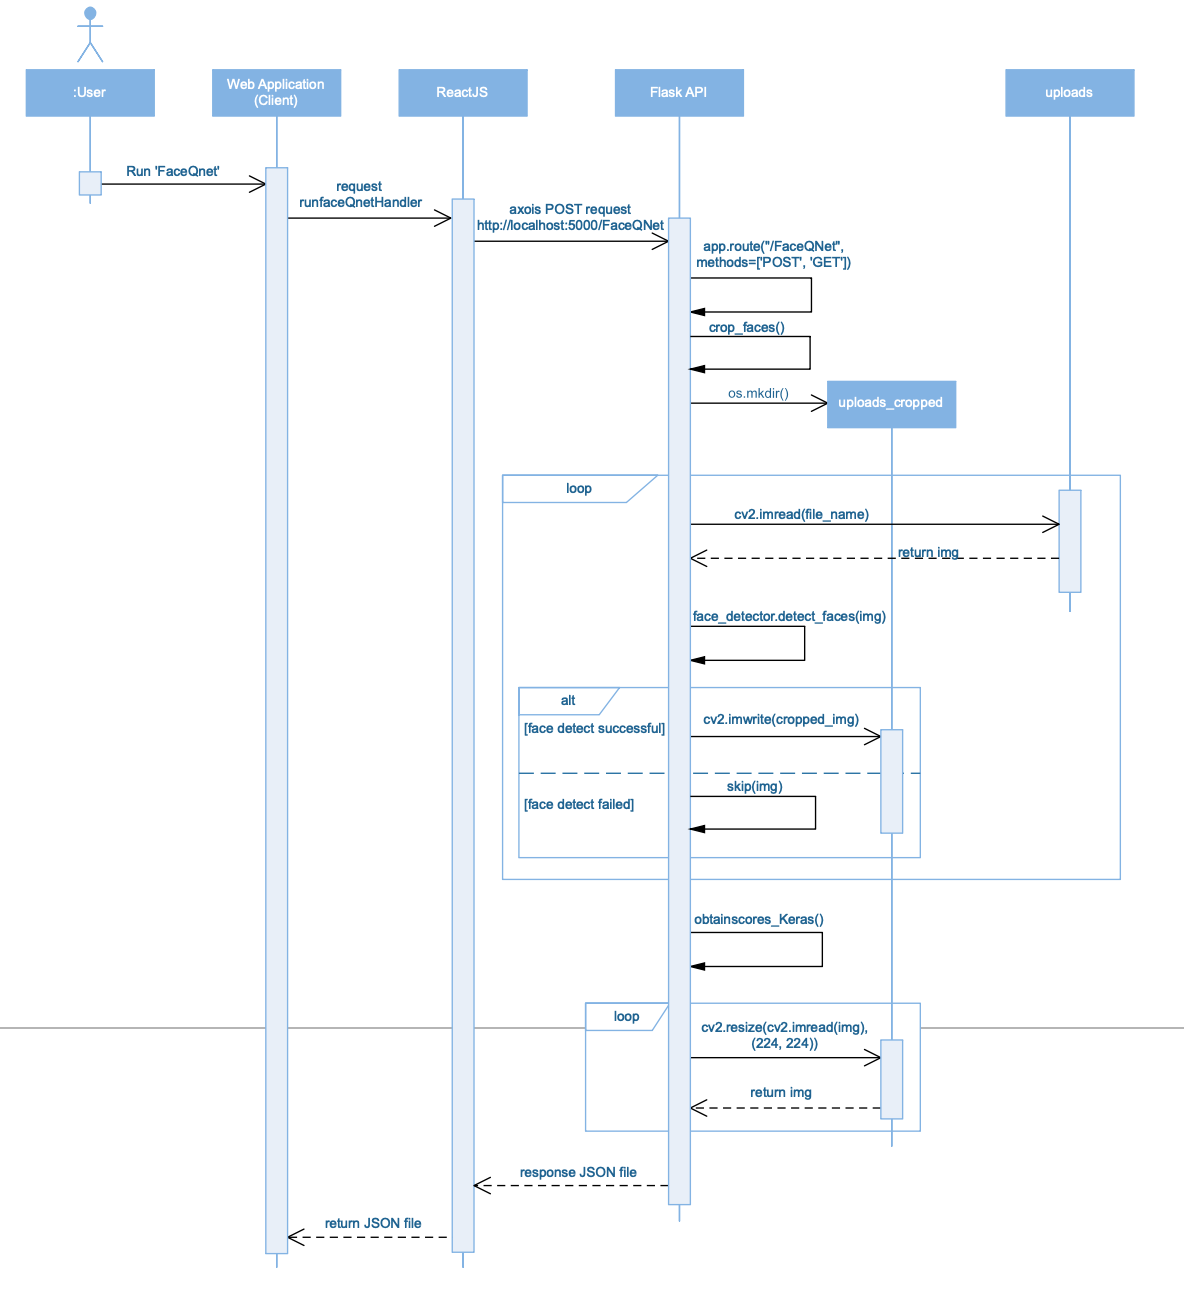
\includegraphics[scale = 0.65]{figures/LowLevel.png}
    \caption{FaceQNet: low level sequence diagram}
    \label{fig:lowlevel}
\end{figure}

Unlike Figure \ref{fig:highlevel}, Figure \ref{fig:lowlevel} in-depth showcases how FaceQNet is executed the first time it is ran on a computer. Before the ``Run 'FaceQnet''' button is clicked in the client, it is given that images have been selected and uploaded to the uploads folder, check Figure \ref{fig:highlevel} to see how this works. Because of that, the uploads-entity already exists instead of being created along the way. The first few steps are quite similar to the previous sequence diagram, however this time an API called FaceQNet is executed that in return starts the FaceQNet FIQM. 
\newpage

The cropping phase of FaceQNet begins, and since this is the first time the API has been called, another folder by the name of uploads\_cropped is created. The function then enters a for-loop that reads all the uploaded images from the original uploads folder, before they are cropped. Unfortunately the cropping tool provided by MTCNN sometimes fails to detect the face in the images which results in an empty image. An alternative scenario then occurs, which ignores these type of images, and they will automatically be provided with the lowest score possible. If no exception happens during the face cropping, the cropped image is saved to the uploads\_cropped folder.  

After having finished the cropping, the API starts the scores prediction, which first has to read all images from the uploads\_cropped folder, resize them and then predict their scores. The metric likewise returns a JSON file with all scores back to the web page. 

\section{Choice of front- and backend}
When choosing development software, we had to take some considerations. First, both backend and frontend software should not be time consuming to master, given that the project consisted of coding and research. Second, it should be uncomplicated to integrate the released FIQMs with the backend as well as creating an intelligible user interface. 

\subsection*{Backend}
The two FIQMs FaceQNet and ISO metrics were written in python. Since we were experienced with python and operated with it in courses throughout the bachelor program, it was natural to choose a python framework for the backend. With a dozen of possible web frameworks, we needed to select a framework which suited our needs in terms of scalability, performance and ease of use. In the end, the choices were between Django and Flask. 

\newpage

\begin{table}[h]
\centering
\resizebox{\textwidth}{!}{%
\begin{tabular}{|l|p{9cm}|} 
\hline
\textbf{Framework} & Django  \\ \hline
\textbf{Advantages} &  Django is a fast framework, making the development process for the developers to increase. It has as high level of scaliability to the users. This feature is the reason many leading websites depend on Django to fulfill their high operational requirements. The framework includes several prebuild development features as user authentication, sitemaps, content administration etc. It has excellent security, preventing the users from several security issues. Django is very flexible as it can be used to create a widely specter of application types. Some of these are social networking such as Instagram or content management systems such as Wagtail \cite{DjangoAdvantages}.     \\ \hline
\textbf{Disadvantages} & First of all, Django has a steep learning curve. Even though it its written in python, it takes a long time for developers to get the hang of it. The framework is considered one of the hardest to master. Django is more suitable for large scale applications rather than smaller products with fewer features and requirements. The unique functionalities within Django can be confusing for developers working with a small project. Djangos' monolithic architecture has a small number of dependencies which make it challenging to use. It does not facilitate developers to utilize python packages and tools, but focuses on code-oriented programming. Django can not provide fast development in terms on requests. Only one request at the time can be fulfilled, meaning it is unable to handle multiple requests concurrently\cite{DjangoDisadvantages}.         \\ \hline
\end{tabular}%
}
\caption{Pros and cons with Django}
\end{table}

\begin{table}[h]
\centering
\resizebox{\textwidth}{!}{%
\begin{tabular}{|l|p{9cm}|}
\hline
\textbf{Framework} & Flask  \\ \hline
\textbf{Advantages} & For programmers with experience in python, it is easy adaptable to work with Flask. This micro framework is simple to manage as there are few standards. Flasks' modular nature let developers instantly create servers and applications, which are distributed across comprehensive networks with certain purposes. It is pliable, meaning that components within the framework are easy to modify, because it is simple to configure. Given that Flask is a micro framework, it has less abstraction layers between the users and the database, cache and requests. This design provide users high level of performance.\cite{DjangoAdvantages}  \\ \hline
\textbf{Disadvantages} & As many beginner web developers tend to use the Flask framework, resulting in low quality code and possibly a bad application. Flask has singular source, meaning that is handles requests in turns. With multiple requests, it could be time consuming to handle the requests. The use of modules in Flask raises security issues. It would be bad if a module contained spiteful data.             \\ \hline
\end{tabular}%
}
\caption{Pros and cons with Flask}
\label{table:a}
\end{table}

Initially, we started the backend development process using Django. This was mainly because the team working with backend had learned about the framework in an earlier course of the bachelor program. However, we eventually concluded not to use Django for the backend. Given some knowledge in the framework, we had not actually developed anything with it. Since Django did not provide the usage of python packages or tools, it would be more time consuming to code the application. The steep learning curve provided by the framework would make the development process even more time consuming. Our project differed in working tasks, by not only have a coding task, made the application smaller in terms of features and requirements. Django was more suitable for larger applications, making the decision of not using the framework clearer. We ended up using Flask for the backend. Immediately after installing the framework, the development productivity increased rapidly. Our python experience was easily adaptable to Flask which made it simple to make a deployable application and integrate FIQMs to the program. 

\subsection*{Frontend}
Given the few requirements and the key concepts of how Mobai wanted the application to be built, simplicity played a big role for us when choosing how to build the frontend. Mobai's vision for the frontend was for it to be a demo to demonstrate some of the key concepts provided by the backend, like uploading images and running FIQMs. The frontend would then be used to easily display results from different FIQMs on a small amount of images, or be used as a demonstration to Mobai's customers. Since we decided to build the frontend as a web application, we quickly understood that is was going to be made out of HTML, CSS and JaveScript.

The backend framework Flask explained in Table \ref{table:a}  has a way of rendering simple HTML pages by itself. In the early stages of our developement, we built a simple HTML page consisting of buttons and text and had Flask render the template. This was a good way of testing the backend functionality. Using this method would simplify the frontend a lot and make the application run solely on the backend port 5000. The problem with this method was that the HTML pages rendered were quite static and had restrictions in form of design and functionality. This also meant that the frontend would be incorporated into the backend, and the backend had to be started in order for the frontend to work. After a discussion with Mobai, we found out that this was not the best solution.

We wanted the frontend to run independently from the backend on its own server. This way, the frontend would not be dependent on the backend to run, and we got more flexibility when it came to design and implementations. We could still code the frontend using basic HTML and some JavaScript, but we found that using a well developed web framework would enhance the design and simplify for future development of the application. Angular and React are the two frameworks we considered to use. 

%write about angular and React

%React is a library for building user interfaces, and can be used to build full stack apps by communicating with a server/api. 

We ended up choosing React, considering its great performance, flexibility and its ability to create dynamic web pages. React has its own Command Line Interface (CLI) tool that makes building a React app easy. This command is called create-react-app and automatically builds up all files, packages and folders that is needed to run a React application. The command also serves the react app with a server using Node.js, which is an open source, cross platform, javaScript runtime environment that gives the ability to run web pages on server side. In order to run the CLI tool, Node.js would have to be installed first. Using this method, a React application could easily be installed and the web page be run on a local server on port 3000 using the Node.js command 'npm start'. This way we have created a frontend independently of the backend running on port 3000. 
%https://en.wikipedia.org/wiki/Node.js
%https://www.youtube.com/watch?v=w7ejDZ8SWv8

%write about material-ui, react hooks,, axios requests

%write about deployment. we dont have to use deployment build, its deployed as a docker container instead, so it can run on port 3000 and 5000 locally. 





\subsection*{Containerization}
One of the main requirements given by Mobai was to deploy the application in a container. With such a containerization \cite{Containerization}, it provided us a lot of benefits:
\begin{itemize}
    \item A container is independent of the operating system, making it portable between dissimilar platforms. 
    \item Containers are efficient in terms of allowing applications being quickly deployed, patched or scaled. 
    \item Containers consume less system overhead than regular hardware or virtual environment owing to that they do not include operating system images. 
    \item It provides better application development, production cycles and testing as containers supports an agile workflow.
    \item Having the application separated into different containers will improve security. 
\end{itemize}

\section{Design and implementation}

\subsection{Flask API}

\section{Testing}

\subsection{User testing}

\subsubsection{Mobai employee}
Send repository to Guoqiang. Get general feedback from him and other people from Mobai.

% Tasks
Deploy the backend and the frontend using Docker.
Upload multiple images.
Run all of metrics at the same time.
Run each of the metrics separately. 
Delete the images uploaded to the backend.
Upload a single image.
Run all of metrics at the same time.
Run each of the metrics separately. 

% General feedback from Mobai

% Add table with problems and solutions. See Viten i senter chapter 9